\documentclass[11pt,a4paper]{article}
\usepackage[margin=1in]{geometry}
\usepackage{tikz}
\usepackage{lmodern}
\usepackage{amsmath}
\usepackage[utf8]{inputenc}
\usepackage{hyperref}
\usepackage{caption}
\usepackage{float}
\newcommand{\uvec}[1]{\boldsymbol{\hat{\textbf{#1}}}}

\title{Using \LaTeX\ for MIT Lecture notes}
\author{Ravi Chhawal}   
\date{October 18, 2023}
\pagenumbering{arabic}

\begin{document}
\maketitle

\begin{enumerate}
      \item \textbf{\LARGE Lecture 1}

            \begin{enumerate}
                  \item \textbf{\Large MIT Introduction to Geometric Viewpoint on physics}
                        \begin{enumerate}
                              \item Mathematical foundations on General Relativity
                              \item Derive Einstein Field Equations
                              \item {\textbf{Spacetime:}} so what is SpaceTime?? from purely mathematical
                                    point of view... A \colorbox{blue!30}{\textbf{manifold}} of events that is \colorbox{blue!30}{\textbf{endowed}} with \colorbox{blue!30}{\textbf{metric}}.
                              \item \textbf{Manifold: }  A set of points with well-understood connectedness property. How we connect on region of space time into another region.(For More rigorous discussion insight please refer Carrol Book on General Relativity.)
                              \item \textbf{Space?????: } Event  When and where something happens. Essentially event is fundamental notion of a coordinate in space and time .
                              \item \textbf{Labels:} i.e coordinates we attach to events,but the event itself is independent on the choice of coordinate system or labels.
                              \item \textbf{Metric:} A notion of distance between events in manifold. Without this, manifold has no notion of distance encoded in it. The idea that the mathematical structure that tells me how far apart the two events are is intimately connected to the properties of gravity.
                              \item \textbf{Special Relativity:} Simplest theory of spacetime, corresponds to general relativity where there is no gravity.
                              \item \textbf{Inertial Reference Frame:} A lattice of clocks and measuring rods that allows us to label-assign coordinates to spacetime events. (\textit{refer to the book of S Thorne on Gravitation}) Is at rest with respect to someone who does not feel any force acting on it.\\
                                    Properties in respect of Inertial Frame of Reference:
                                    \begin{enumerate}
                                          \item This lattice moves freely through spacetime, No force acting in it, is not rotating.
                                          \item Measuring rods are orthogonal wrt each other. i.e. orthogonal coordinate system.
                                          \item Spacing system of measurement are uniformly ticked. Tick mark are uniformly spaced.
                                          \item clocks tick uniformly
                                          \item Clock Synchronized using \textbf{"Einstein Synchronization Procedure"}
                                    \end{enumerate}
                                    This procedure takes advantage of the fact that the speed of light is same for all frame of reference (observers). Speed of light is key invariant irrespective of any frame of reference.
                                    \begin{figure}[H]
                                          \centering
                                          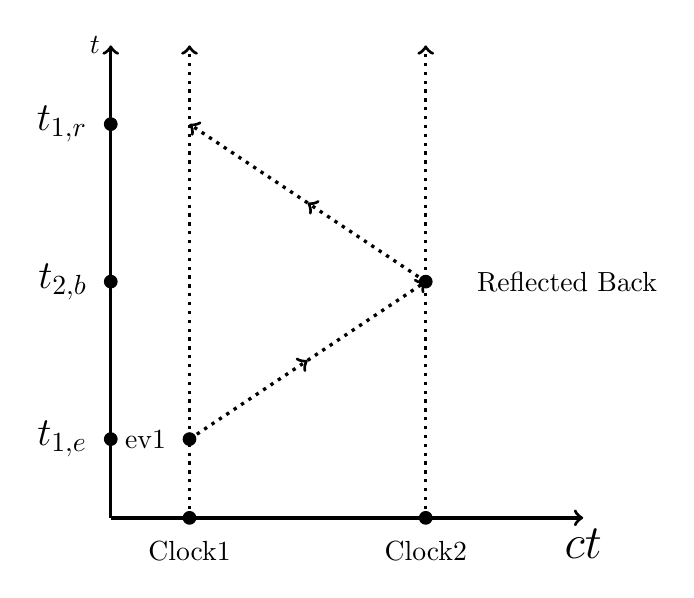
\begin{tikzpicture}[scale=2]
                                                \draw[->,very thick] (0,0) -- (3,0)node[below] {\fontsize{19}{0}$ct$};
                                                \draw[->,very thick] (0,0) -- (0,3)node[left] {$t$};
                                                \draw[->,very thick,dotted] (0.5,0) -- (0.5,3)node[below] {$$};
                                                \draw[->,very thick,dotted] (2,0) -- (2,3)node[below] {$$};
                                                \draw[->,very thick,dotted] (.5,.5)--(1.25,1) node[below] {$$};
                                                \draw[->,very thick,dotted] (1.25,1) -- (2,1.5)node[below] {$$};
                                                \draw[->,very thick,dotted] (2,1.5)--(1.25,2) node[below] {$$};
                                                \draw[->,very thick,dotted] (1.25,2) -- (0.5,2.5)node[below] {$$};
                                                %\draw[step=.5cm,gray,very thin] (0,-0) grid (2.9,2.9);
                                                \filldraw (.5,0) circle (0.04)node[below=5pt]{Clock1};
                                                \filldraw (.5,0.5) circle (0.04)node[left=5pt]{ev1};
                                                \filldraw (2,0) circle (0.04)node[below=5pt]{Clock2};
                                                \filldraw (2,1.5) circle (0.04)node[right=15pt]{Reflected Back};
                                                \filldraw (0,.5) circle (0.04)node[left=5pt,font = {\Large\bfseries}]{${t_{1,e}}$};
                                                \filldraw (0,2.5) circle (0.04)node[left=5pt,font = {\Large\bfseries}]{${t_{1,r}}$};
                                                \filldraw (0,1.5) circle (0.04)node[left=5pt,font = {\Large\bfseries}]{${t_{2,b}}$};
                                          \end{tikzpicture}
                                          \caption{} \label{Fig.1}
                                    \end{figure}
                                    $t_{1,e}$: Event When Clock1 emits light pulse.\\
                                    $t_{2,b}$: Event When observer at Clock2 reflects light pulse.\\
                                    $t_{1,r}$: Event When Clock1 receives reflected light pulse.\\
                                    $t_{2,b}=\displaystyle{\frac{t_{1,e}+t_{1,r}}{2}}$\\
                        \end{enumerate}
                  \item \textbf{\Large Geometric Viewpoint on physics}
                        \begin{enumerate}
                              \item \textbf{Units}
                                    \begin{itemize}
                                          \item \textbf{Units:} Choose basic unit of length to be the distance light travels in basic unit of time.
                                          \item $\Rightarrow$ If my basic unit of time is 1 sec then basic unit of length will be one light second
                                          \item Further if we take unit time to be one nano sec then corresponding unit length will be 1 foot \textit{i.e. speed of light is 1 foot per nano sec}
                                          \item we take speed of light to be one unit $c=\displaystyle{\frac{\text{1 light time unit}}{\text{time unit}}}$
                                          \item This means that all velocities will be dimensionless
                                    \end{itemize}
                                    \vspace{11pt}
                                    \begin{figure}[H]
                                          \centering
                                          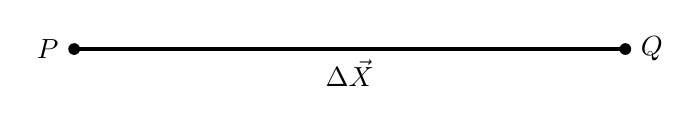
\begin{tikzpicture}
                                                \draw[very thick] (0,0)--node[below]{$\Delta \vec{X}$} ++ (7,0);
                                                \node[outer sep=0pt,circle, fill,inner sep=1.5pt,label={[fill=white]left:$P$}] (P) at (0,0) {};
                                                \node[outer sep=0pt,circle, fill,inner sep=1.5pt, label={[fill=white]right:$Q$}] (Q) at (7,0) {};
                                          \end{tikzpicture}%
                                          \caption{} \label{Fig.2}
                                    \end{figure}
                                    $\Delta \vec{X}$ is displacement in space time from point $P$ to $Q$\\
                                    We Shall define components with respect to observer $O$.
                                    \begin{center}
                                          $\Delta \vec{X} \mathop = \limits^{\boldsymbol{\cdot}}_{O} \left(t_Q-t_P,X_Q-X_P,Y_Q-Y_P,Z_Q-Z_p\right)$\\
                                    \end{center}
                                    The above equation can be written in compact notation i.e\\
                                    $\Delta \vec{X} \mathop \rightarrow \limits^{}_{O} \Delta {X^{\mu}}$\\
                                    where $\mu \in \left[ t,x,y,z\right]$ or  $\mu \in \left[ 0,1,2,3\right]$\\
                                    Usually 0 corresponds to time whereas 1,2,3 may denote other orthogonal coordinate system.\\
                              \item \textbf{Different Inertial Observer:}\\
                                    $P$ $Q$ and $\Delta \vec{X}$ are geometric objects exists independent of representation.\\
                                    $\Delta \vec{X} \mathop \rightarrow \limits^{}_{\overline{O}} \Delta {X^{\overline{\mu}}}$\\
                                    $O$ and $\overline{O}$ components are related by lorentz transformation as given below:\\
                                    $\Delta {X^{\overline{0}}}=\gamma {\Delta X^0} - \gamma\ v\ {\Delta X^1}$\\
                                    $\Delta {X^{\overline{1}}}=-\gamma\ v\ {\Delta X^0} + \gamma{\Delta X^1}$\\
                                    $\Delta {X^{\overline{2}}}={\Delta X^2}$\\
                                    $\Delta {X^{\overline{3}}}={\Delta X^3}$\\
                                    The above set of transformation holds good for reference frame $\overline{O}$ moving along axis 1 with speed $v$ along axis 1 as seen by observer $O$.\\
                                    where $\gamma  = \left[\frac{1}{\sqrt{1-v^2}}\right]$\\
                                    here $v$ is light speed unit as defined earlier.\\
                                    Better compact notation:\\
                                    \[\Delta X^{\overline{\mu}}=\sum_{\nu = 0}^{3}\Lambda^{\overline{\mu}}_{\nu}\ \Delta X^{\nu}\]
                                    or  writing in simple way of Einstein Summation convention: Repeated indices in upstairs and downstairs positions are summed from 0 to 3.
                                    \[\Delta X^{\overline{\mu}}=\Lambda^{\overline{\mu}}_{\nu}\ \Delta X^{\nu}\]
                                    \[\Lambda^{\overline{\mu}}_{\nu}=\frac{\delta X^{\overline{\mu}}}{ \delta X^{\nu}}\]
                                    the above equation will be used in transformation from one reference frame to other.\\
                                    $\nu$ is dummy index, however $\overline{\mu}$ is not the dummy index sometimes called free index.
                              \item \textbf{Spacetime Vector:}
                                    Any quartet of numbers (i.e components) which transforms between Inertial reference Frame like displacement Vector.\\
                                    $\vec{A} \mathop = \limits^{}_{O} \left(A^0,A^1,A^2,A^3\right)\mathop \rightarrow \limits^{}_{O} {A^{\alpha}}$\\
                                    If $A^{\overline{\mu}}=\Lambda^{\overline{\mu}}_{\alpha}.A^{\alpha}$\\ decides the component of Vector with respect to observer $O$ then, it also requires linearity rules\\
                                    i.e If $\vec{A}$ and $\vec{B}$ are two vectors then their sum\\
                                    $\vec{C}=\vec{A}+\vec{B}$\\
                                    is also a vector.\\
                                    Further if $\vec{A}$ is a vector and $a$ is a scaler then their product is a vector.\\
                                    $\vec{D}=a.\vec{A}$\\
                                    \textbf{Note:} the scaler quantity should be same for all frame of reference/observers. This means mass cannot be taken as scaler.

                        \end{enumerate}
            \end{enumerate}
      \item \textbf{\LARGE Lecture 2}
            \begin{enumerate}
                  \item \textbf{Introduction to Tensors}\\
                        \textbf{Basis Vector:} In Frame of reference/observer '$O$' we can write down 4 special vectors :\\
                        $\vec e_0 \mathop = \limits^{}_{O} (1,0,0,0)$\\
                        $\vec e_1 \mathop = \limits^{}_{O} (0,1,0,0)$\\
                        $\vec e_2 \mathop = \limits^{}_{O} (0,0,1,0)$\\
                        $\vec e_3 \mathop = \limits^{}_{O} (0,0,0,1)$\\
                        Compact way of writing this:\\
                        $(\vec e_{\alpha})^{\beta}\mathop = \limits^{}_{O}  \delta^{\beta}_{\alpha}$\\
                        \textbf{Kronecker delta function}\\
                        The utility os above set of equations is:\\
                        $\vec{A}=A^{\alpha}.\vec{e}_{\alpha}$\\
                        The above equation represents actual equality and not representation symbol.\\
                        we shall now see how basis vectors transforms when reference frame changes.
                        \begin{flalign*}
                              \vec{A}=A^{\alpha}.\vec{e}_{\alpha} & =A^{\overline{\mu}}.\vec{e}_{\overline{\mu}}                                     & \\
                                                                  & =\left(\Lambda^{\overline{\mu}}_{\beta}A^{\beta} \right)\vec{e}_{\overline{\mu}}
                        \end{flalign*}
                        \textbf{Index Notation}\\
                        Normally the above equation is represented in matrix notation. However as the index of matrix increases representation in matrix form is not desirable.\\
                        For ordinary multiplication the above equation can be reformatted as\\
                        $=\left(A^{\beta} \Lambda^{\overline{\mu}}_{\beta} \right)\vec{e}_{\overline{\mu}}$\\
                        In above equation $\beta$ is dummy index and can be re-written as...\\
                        $A^{\alpha}.\vec{e}_{\alpha} = A^{\beta}  \Lambda^{\overline{\mu}}_{\beta}\vec{e}_{\overline{\mu}}$\\
                        $\Rightarrow A^{\alpha}.\vec{e}_{\alpha} = A^{\alpha}  \Lambda^{\overline{\mu}}_{\alpha}\vec{e}_{\overline{\mu}}$\\
                        $\Rightarrow A^{\alpha}.\vec{e}_{\alpha} - A^{\alpha}  \Lambda^{\overline{\mu}}_{\alpha}\vec{e}_{\overline{\mu}}=0$\\
                        $\Rightarrow A^{\alpha}\left(\vec{e}_{\alpha} - \Lambda^{\overline{\mu}}_{\alpha}\vec{e}_{\overline{\mu}}\right)=0------------------(1)$\\
                        Since $A^{\alpha}$ is arbitrary... the above equation (1) will hold good or are valid only if\\
                        $\vec{e}_{\alpha} = \Lambda^{\overline{\mu}}_{\alpha}\vec{e}_{\overline{\mu}}$\\
                        since $A^{\overline{\mu}}=\Lambda^{\overline{\mu}}_{\alpha}.A^{\alpha}$\\
                        to get inverse lorentz transformation just reverse the velocity components\\

                        $\vec{e}_{\alpha} = \Lambda^{\overline{\mu}}_{\alpha}(\underset{\sim}{v})\vec{e}_{\overline{\mu}}$\\

                        $\vec{e}_{\overline{\mu}} = \Lambda^{\nu}_{\overline{\mu}}(-\underset{\sim}{v})\vec{e}_{\nu} $\\

                        Using the transformation:\\
                        $\vec{e}_{\alpha} = \Lambda^{\overline{\beta}}_{\alpha}(\underset{\sim}{v})\vec{e}_{\overline{\beta}}$\\
                        $\vec{e}_{\alpha} = \Lambda^{\overline{\beta}}_{\alpha}(\underset{\sim}{v})\left[\Lambda^{\gamma}_{\overline{\beta}}(-\underset{\sim}{v})\vec{e}_{\gamma}\right]$\\
                        $\vec{e}_{\alpha} = \left[\Lambda^{\overline{\beta}}_{\alpha}(\underset{\sim}{v})\, \Lambda^{\gamma}_{\overline{\beta}}(-\underset{\sim}{v})\right]\vec{e}_{\gamma}$\\
                        the above equation will hold good if the components under square brackets reduces to Identity matrix.\\
                        kronecker delta function:\\
                        $\delta^{\alpha}_{\gamma}= \Lambda^{\overline{\beta}}_{\alpha}\, \Lambda^{\gamma}_{\overline{\beta}}$\\
                        likewise:\\
                        $\delta^{\overline\alpha}_{\overline\gamma}= \Lambda^{\beta}_{\overline\alpha}\, \Lambda^{\overline\gamma}_{\beta}$\\

                        we shall now see operations which can be done with these 4 vectors (i.e 3 space vector and one time vector)
                        \begin{enumerate}
                              \item \textbf{Scaler Product:}\\
                                    As per special relativity\\
                                    $\Delta{S^2}=-\Delta{t^2}+\Delta{X^2}+\Delta{Y^2}+\Delta{Z^2}$\\
                                    this is invariant: Same in all lorentz frame of reference\\
                                    the above equation can be written as\\
                                    $\Delta{S^2} = \Delta \vec{X} \cdot \Delta\vec{X}$\\
                                    $\mathop = \limits^{.}_{\theta}  -(\Delta{X_0})^2+(\Delta{X_1})^2+(\Delta{X_2})^2+(\Delta{X_3})^2$\\
                                    The question may arise that why the first component i.e time has negative sign where as other dimensions i.e spacial direction are +ve sign. The direction of time is one-sided. we cannot go back and forth in time. This is how the space time as we know it. It is part of built-in geometry of nature.\\
                                    this has same transformation properties as displacement vector.\\
                                    since 4 vectors have same transformation properties as $\Delta \vec{X}$, we similarly define\\
                                    $\vec{A}\cdot\vec{A} \mathop = \limits^{.}_{\theta} - (A^0)^2 + (A^1)^2+ (A^2)^2+ (A^3)^2$\\
                                    because this transformation has same properties as displacement vector then this equation must be lorentz invariant.

                              \item \textbf{Terminology:}\\
                                    If $\vec{A}\cdot\vec{A} < 0$ then vector $\vec{A}$ is \textbf{"time like"}.\\
                                    If $\vec{A}\cdot\vec{A} > 0$ then vector $\vec{A}$ is \textbf{"Space like"}.\\
                                    If $\vec{A}\cdot\vec{A} = 0$ then vector $\vec{A}$ is \textbf{"light like or NULL"}.\\
                              \item \textbf{More General Notation}\\
                                    Scaler is a quantity which does not have any component\\
                                    $\vec{A}\cdot\vec{B} \mathop = \limits^{.}_{\theta} - A^0\cdot B^0 + A^1\cdot B^1 + A^2\cdot B^2 + A^3\cdot B^3$\\
                                    This quantity must also be an invariant. This can be easily proved by using $\vec{C}=\vec{A}+\vec{B}$, since $\vec{C}\cdot\vec{C}$ is invariant\\
                                    $\Rightarrow$ $ \vec{A}\cdot\vec{B}$ is also lorentz invariant.\\
                                    using $\vec{A}$ and $\vec{B}$ as component of basis vectors we have
                                    \begin{align*}
                                          \vec{A}\cdot\vec{B} & = (A^{\alpha}\vec{e_{\alpha}})\cdot(B^{\beta}\vec{e_{\beta}}) \\
                                                              & = A^{\alpha}.B^{\beta} (\vec{e_{\alpha}}.\vec{e_{\beta}})     \\
                                                              & = A^{\alpha}.B^{\beta} {\displaystyle{\eta_{\alpha\beta}}}
                                    \end{align*}
                                    here ${\displaystyle{\eta_{\alpha\beta}}}$ is two index tensor
                                    \[ {\displaystyle{\eta_{\alpha\beta}}} = \begin{pmatrix}
                                                -1 & 0 & 0 & 0 \\
                                                0  & 1 & 0 & 0 \\
                                                0  & 0 & 1 & 0 \\
                                                0  & 0 & 0 & 1 \\\end{pmatrix} \rightarrow the\ "metric"\ Tensor \]
                                    $\Delta{S^2} = \Delta \vec{X} \cdot \Delta\vec{X}$\\
                                    $\Rightarrow \Delta{S^2} = {\displaystyle{\eta_{\alpha\beta}}} \Delta X^{\alpha} \Delta X^{\beta}$\\
                                    we will use $\eta$ for transformation in cartesian coordinates\\
                                    rewriting the above equations in form of differentials we have\\
                                    $d{S^2} = d \vec{X} \cdot d\vec{X}$\\
                                    $\Rightarrow d {S^2} = {\displaystyle{\eta_{\alpha\beta}}}\ d X^{\alpha}\ d X^{\beta}$\\

                                    when the equation below holds true: i.e\\
                                    $d\vec{X}= dX^{\alpha}\ \vec{e}_{\alpha}$\\
                                    then we say that $\vec{e}_{\alpha}$ is \textbf{coordinate basis} vector.
                              \item \textbf{Curvilinear coordinates}:\\
                                    $d\underset{\sim}{X} = dX^i \vec{e_i}$\\
                                    $= d{r}\ \vec{e_r} + d\theta\ \vec{e_{\theta}} +d\phi\ \vec{e_{\phi}} $\\
                                    $= d{r}\ \vec{e}_{\hat{r}} + d\theta\ r \vec{e}_{\hat{\theta}} +d\phi\ r \sin\theta\ \vec{e}_{\Hat{\phi}} $\\

                                    $\vec{e}_{\Hat{i}}$ is orthogonal basis if \\
                                    $\vec{e}_{\Hat{i}}\cdot \vec{e}_{\Hat{j}} = \delta_{ij}$\\
                                    kronecker delta function.\\
                                    for Curvilinear coordinates as defined above this is not the case as :\\
                                    $\vec{e}_{\hat{r}} \cdot \vec{e}_{\hat{r}} = 1 $\\
                                    $\vec{e}_{\hat{\theta}} \cdot \vec{e}_{\hat{\theta}} = r^2 $\\
                                    $\vec{e}_{\hat{\phi}} \cdot \vec{e}_{\hat{\phi}} = r^2.\sin^2\theta $\\
                                    thus the metric tensor ${\displaystyle{\eta_{\alpha\beta}}}$ will change for Curvilinear coordinate system as we are not dealing with orthonormal basis vectors.

                              \item \textbf{Important 4 vectors}\\
                                    $\vec{U}\equiv  \dfrac{d\vec{X}}{dT}$ this has 4 velocity components..\\
                                    $dT$ is time interval as measured along the trajectory of the observer \\
                                    Interval of \textbf{"proper time"}\\
                                    for observer seeing an object going by with a constant velocity. he wil observer 4 velocity components given by :\\
                                    $\mathop = \limits^{o}_{} (\gamma,\gamma \underset{\sim}{V})$\\
                                    where $\gamma$ is lorentz factor given by $\dfrac{1}{\sqrt{1-v^2}}$\\
                                    In rest frame of the observer $\vec{u} = (1,\underset{\sim}{0})$\\
                                    i.e person is standing still but moving through time.\\
                              \item \textbf{4 Momentum} components\\
                                    $\vec{P} = m \vec{u}$ where $m$ is \textbf{"rest mass"} of the object\\
                                    External observer will see two components\\
                                    $\mathop = \limits^{\cdot}_{} (E,P)$\\
                                    scaler product $\vec{u} \cdot \vec{u} = -\gamma^2 + \gamma^2.v^2 = -1$\\
                                    a) if $v=0$ then $\gamma=1$ the above equation will hold good/true.\\
                                    b) $\gamma$ is frame invariant quantity this means transformation equations shall hold good for any frame of reference we shall use this property to solve complex equations.\\
                                    c) Now for 4-Momentum components just multiply 4-velocity components times mass of the object.\\
                                    $\vec{p} \cdot \vec{p}=m^2\ \vec{u} \cdot \vec{u} = -m^2$\\
                                    Since the above equation is also related to energy and Momentum we have\\
                                    $=-E^2 + \lvert P \rvert^2$\\
                                    or \\
                                    $E^2 - \lvert P \rvert^2 = m^2$\\
                                    in the above equation we have taken velocity of light in free space "c=1" as unit length...a more general form will be....\\
                                    $E^2 -  P^2 \cdot c^2= m^2\cdot c^4$\\
                              \item \textbf{Conservation of 4-Momentum}\\
                                    we have N particles interacting, then we have\\
                                    \[\vec{P}_{TOT}= \sum_{i=0}^{N}\vec{p}_{i}\]
                                    the total Momentum is conserved in this interaction.\\
                                    Algebra often simplifies by choosing a convenient frame of reference...\\
                                    i.e. \textbf{Center of Momentum} frame...\\
                                    \[\vec{P}_{TOT} \mathop = \limits^{\cdot}_{CoM} (E,\underset{\sim}{0})\]
                                    Zero special momentum.......\\
                                    this is specially relevant/useful of we are studying particle collision\\
                                    very useful results follows from invariance of scaler product...\\
                                    let $\vec{p}$ be the 4-Momentum of the particle A\\
                                    testing123


                        \end{enumerate}
            \end{enumerate}
\end{enumerate}
\noindent\rule{\textwidth}{1pt}
\href{https://youtu.be/TiHHz3sKDbY?list=PL6Q1107aDr%SgQ1DBEugejXLfQX76hfSnX&t=1188}{text} Draw.io
\end{document}

%https://youtu.be/TiHHz3sKDbY?list=PL6Q1107aDrSgQ1DBEugejXLfQX76hfSnX&t=3510
%Format Document SHift+Alt+F